\chapter{Introduction}\label{chapter:1}

%------------------------------------------------------------%
%------------ Introduction to The Field/Context -------------%
%------------------------------------------------------------%

\section{Formation Flight}
	Scientist have long looked to nature for inspiration; the field of biomimicry is devoted to developing techniques to emulate nature's strategies. One motivating example is how geese, and other migratory birds, fly in a `V' formation \cite{Gould1974,Hainsworth1989,Cutts1994,Weimerskirch2001,Portugal2014} when travelling long distances. Key research shows that birds participating in such formations will have significant increases to their range \cite{Lissaman1970,Cutts1994} while exhibiting lower heart rates \cite{Weimerskirch2001} during flight compared to flying alone. 


		\begin{figure}[ht]
		\centering
		\subfigure[Top-Down View]{
		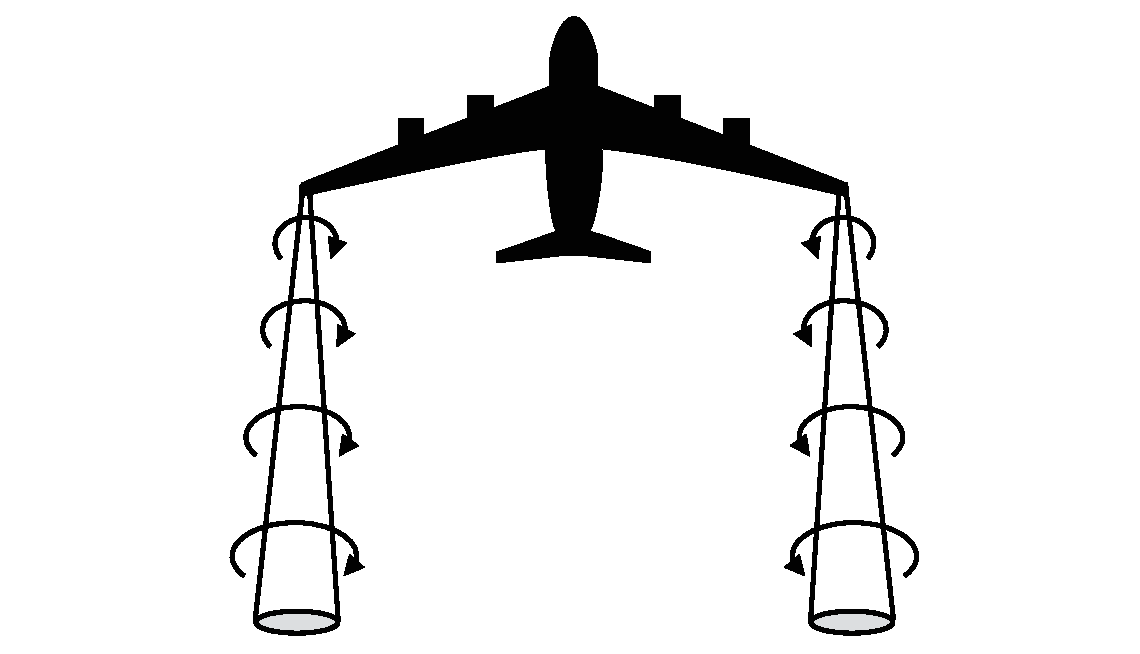
\includegraphics[width= 0.65 \columnwidth]{Chapter01/figures/wake-vortex-top.eps}
		\label{fig:vortex-top}
		}
		\subfigure[Rear view]{
		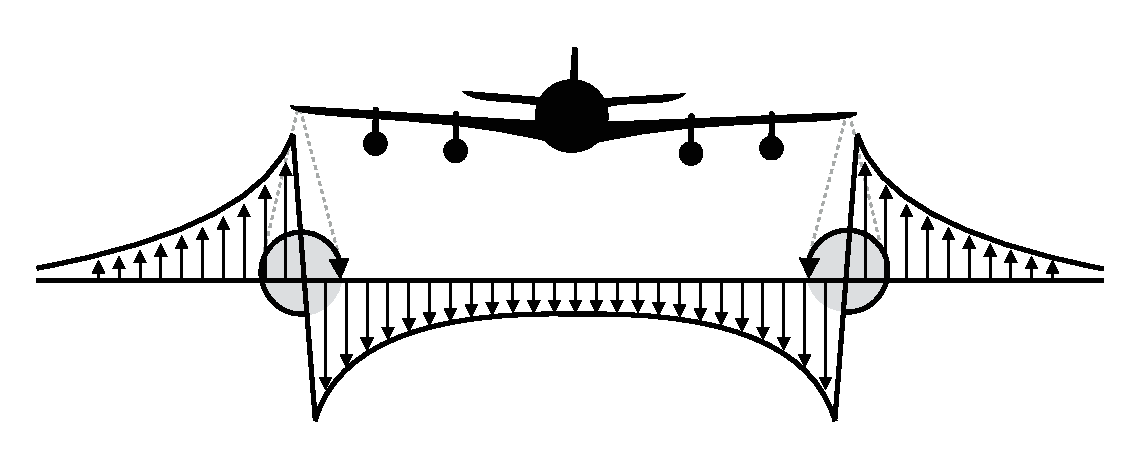
\includegraphics[width= 0.65 \columnwidth]{Chapter01/figures/wake-vortex-rear.eps}
		\label{fig:vortex-rear}
		}
		\caption[Wing-tip vortices and regions of upwash and downwash]{Wing-tip vortices and regions of upwash and downwash}\label{fig:vortices}
		\end{figure}

	The aerodynamic fundamentals behind formation flight for aircraft are fairly well studied \cite{Okolo2014,Pahle2012,Ning2011,Liu2015,Blake2004a}. As an aircraft flies, the pressure differentials created over the wings' surface, generates lift. The wake left behind the lifting-wing induces downwash inboard, between the aircraft wingtips, and a corresponding upwash outboard as depicted in \Cref{fig:vortices}. A trailing aircraft flying through this region of upwash can maintain its flight while operating at a lower apparent angle of attack, that is, a lower angle of attack relative to the horizon. Therefore the aircraft observes a significant reduction in induced drag and as a result a corresponding reduction in fuel burn. 




